\documentclass{standalone}
\usepackage{tikz}
\usetikzlibrary{decorations.markings}

\begin{document}
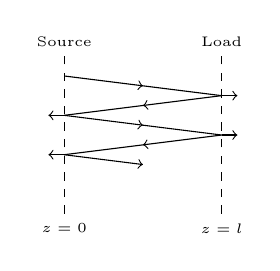
\begin{tikzpicture}[scale=0.5]
    \begin{scope}[thin,decoration={
        markings,
        mark=at position 0.5 with {\arrow{>}}}
        ]
        \draw[dashed] (-2,-2)node[anchor=north,font=\tiny]{$z=0$} -- (-2,2)node[anchor=south,font=\tiny]{Source};
        \draw[dashed] (2,-2)node[anchor=north,font=\tiny]{$z=l$} -- (2,2)node[anchor=south,font=\tiny]{Load};
        \draw[postaction={decorate}] (-2,1.5) -- (2,1);
        \draw[->] (2,1) -- (2.4,1);
        \draw[postaction={decorate}] (2,1) -- (-2,0.5);
        \draw[->] (-2,0.5) -- (-2.4,0.5);
        \draw[postaction={decorate}] (-2,0.5) -- (2,0);
        \draw[->] (2,0) -- (2.4,0);
        \draw[postaction={decorate}] (2,0) -- (-2,-0.5);
        \draw[->] (-2,-0.5) -- (-2.4,-0.5);
        \draw[->] (-2,-0.5) -- (0,-0.75);
    \end{scope}

\end{tikzpicture}
\end{document}